% Compte rendu Phytopathologie (M1, 2023-2024). Compiler dans outils/rapports/rouille : ../compiler.sh rouille
\documentclass[11pt,a4paper]{article}
\usepackage{../rapport-portfolio}
\definecolor{themehex}{HTML}{A9471F}\colorlet{theme}{themehex}
\addbibresource{references.bib}

\titrerapport{Rouille du peuplier et diagnostic des maladies des végétaux}
\titrecourt{Rouille du peuplier et diagnostic}
\soustitre{Pathotypage de \emph{Melampsora larici-populina} et 24 fiches de reconnaissance de bioagresseurs}
\auteurs{Jérémy Genty et Garance Delmas}
\cadre{Master 1 AETPF BICG · UE Phytopathologie · Université d'Orléans}
\annee{Compte rendu de travaux pratiques · 2023-2024}
\motcle{Santé des végétaux}
\visuel{\photogarde{figures/s19_2.jpg}}
\creditvisuel{Pustules de rouille sur une feuille de peuplier, observées à la loupe binoculaire.}

% Fiche de diagnostic : \fiche{titre}{photos}{agent}{hote}{symptomes}{remarque ou vide}
\newcommand{\fiche}[6]{%
  \needspace{15\baselineskip}%
  \subsection{#1}
  \begin{center}#2\end{center}\vspace{-2mm}
  {\small\begin{tabularx}{\linewidth}{@{}>{\bfseries\color{theme}}l@{\hspace{4mm}}X@{}}
  Agent & #3\\ Hôte & #4\\ Symptômes & #5\\
  \end{tabularx}}%
  \if\relax\detokenize{#6}\relax\else\par{\small\color{gris}#6}\par\fi
  \vspace{2mm}}
\newcommand{\ph}[1]{\includegraphics[height=30mm,width=0.32\linewidth,keepaspectratio]{figures/#1}\hspace{1.5mm}}

\begin{document}
\pagedegarde

\enbref{La souche 14AA36 de rouille du peuplier porte les virulences 1, 3, 4, 5 et 7 : elle contourne les résistances correspondantes. Deux clones de résistance inconnue (Fabre2 et Fabre4) lui résistent, deux autres y sont sensibles. La souche 98AG69 reste ininterprétable, faute d'infection du témoin. La seconde partie rassemble 24 fiches de diagnostic : champignons, insectes et acariens, plantes parasites, bactéries et virus.}

\section{Pathotypage de souches de rouille du peuplier}
\subsection{Contexte et objectif}
Le peuplier est une essence majeure de la production de bois d'œuvre en France. Sa principale maladie foliaire, la rouille due à \emph{Melampsora larici-populina}, réduit la photosynthèse, la croissance et l'aoûtement des rameaux. Les cultivars plantés reposent souvent sur des résistances totales, de type gène pour gène : chaque gène de résistance (R) bloque les souches qui ne portent pas la virulence correspondante. Dès qu'une souche acquiert cette virulence, la résistance est contournée \parencite{pinon2005}.

Huit virulences sont connues chez \emph{M. larici-populina}, repérées grâce à une gamme de clones différentiels portant chacun un gène R. Le pathotype d'une souche est la liste des virulences qu'elle porte. Ce TP visait à établir le pathotype des souches 98AG69 et 14AA36 (partie~1.2), puis à tester des clones de résistance inconnue face à ces souches (partie~1.3).

\subsection{Pathotypage des souches}
\subsubsection{Dispositif}
Une suspension de spores (1~mg/15~mL d'eau osmosée) est pulvérisée sur des disques de feuilles des clones différentiels (figure~\ref{fig:dispositif}). Le clone Robusta, sensible à toutes les souches, sert de témoin positif : sans sores sur Robusta après 14 jours, le test n'est pas interprétable. Chaque disque est noté selon le nombre de sores (classe 0 : aucun ; 1 : moins de 10 ; 2 : 10 à 30 ; 3 : 30 à 60 ; 4 : plus de 60) et leur taille (petits, moyens ou grands).

\begin{figure}[ht]
\centering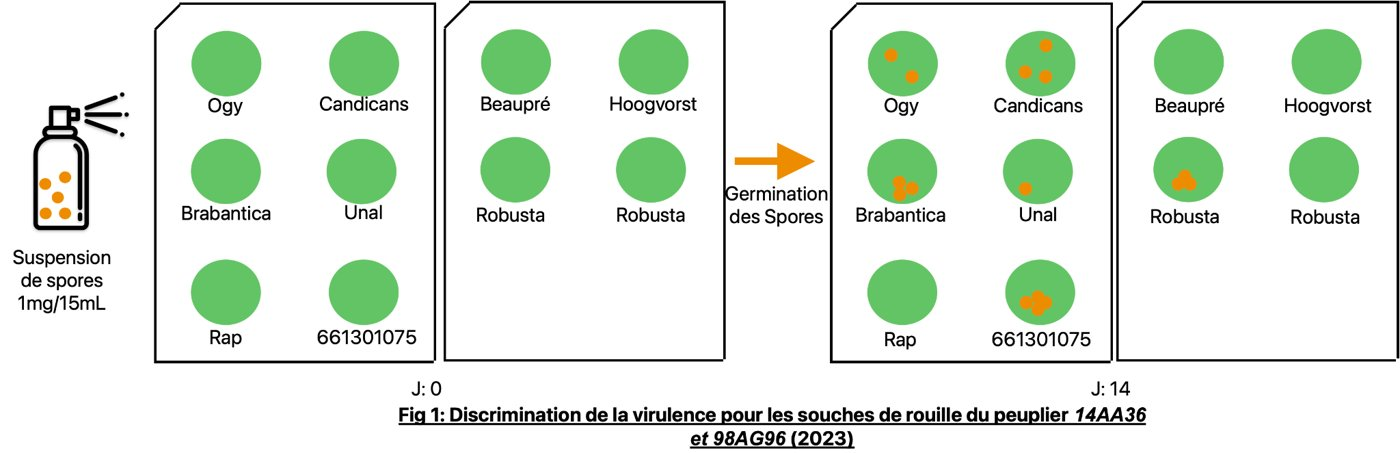
\includegraphics[width=0.85\linewidth]{figures/s03_1.jpg}
\caption{Dispositif de pathotypage : inoculation des disques foliaires des clones différentiels, puis lecture à 14 jours.}
\label{fig:dispositif}
\end{figure}

\subsubsection{Résultats}
Les inoculations de 2023 n'ont pas pu être lues, les spores ayant été mal conservées. Nous avons donc interprété les tests des années précédentes : 2020 et deux séries de 2021, la série~1 de 2021 n'étant pas retenue pour 98AG69 (tableau~\ref{tab:patho}, figure~\ref{fig:plaques}).

\begin{table}[ht]
\centering\small
\caption{Pathotypage : classe de nombre de sores et taille (p : petits, m : moyens, g : grands) par clone différentiel, souche et série.}
\label{tab:patho}
\begin{tabular}{@{}llccccc@{}}
\toprule\entete
 & & \multicolumn{3}{c}{14AA36} & \multicolumn{2}{c}{98AG69}\\
\cmidrule(lr){3-5}\cmidrule(l){6-7}\entete
Clone & Rôle & 2020 & 2021.1 & 2021.2 & 2020 & 2021.2\\
\midrule
Robusta & témoin universel & \textbf{4 p} & 0 & 0 & 0 & 0\\
Ogy & virulence 1 & 2 p & 0 & 1 p & 2 m & 0\\
Candicans × Aurora & virulence 2 & 0 & 0 & 0 & 0 & 2 p\\
Brabantica & virulence 3 & 1 p & 2 p & 1 p & 0 & 0\\
Unal & virulence 4 & 3 m & 0 & 1 p & 2 m & 0\\
Rap & virulence 5 & 4 g & 0 & 0 & 3 p & 0\\
661301075-84B09 & virulence 6 & 0 & 0 & 0 & 1 m & 0\\
Beaupré & virulence 7 & 1 p & 1 p & 0 & 0 & 1 m\\
Hoogvorst & virulence 8 & 0 & 0 & 0 & 0 & 0\\
\bottomrule
\end{tabular}
\end{table}

\begin{figure}[ht]
\centering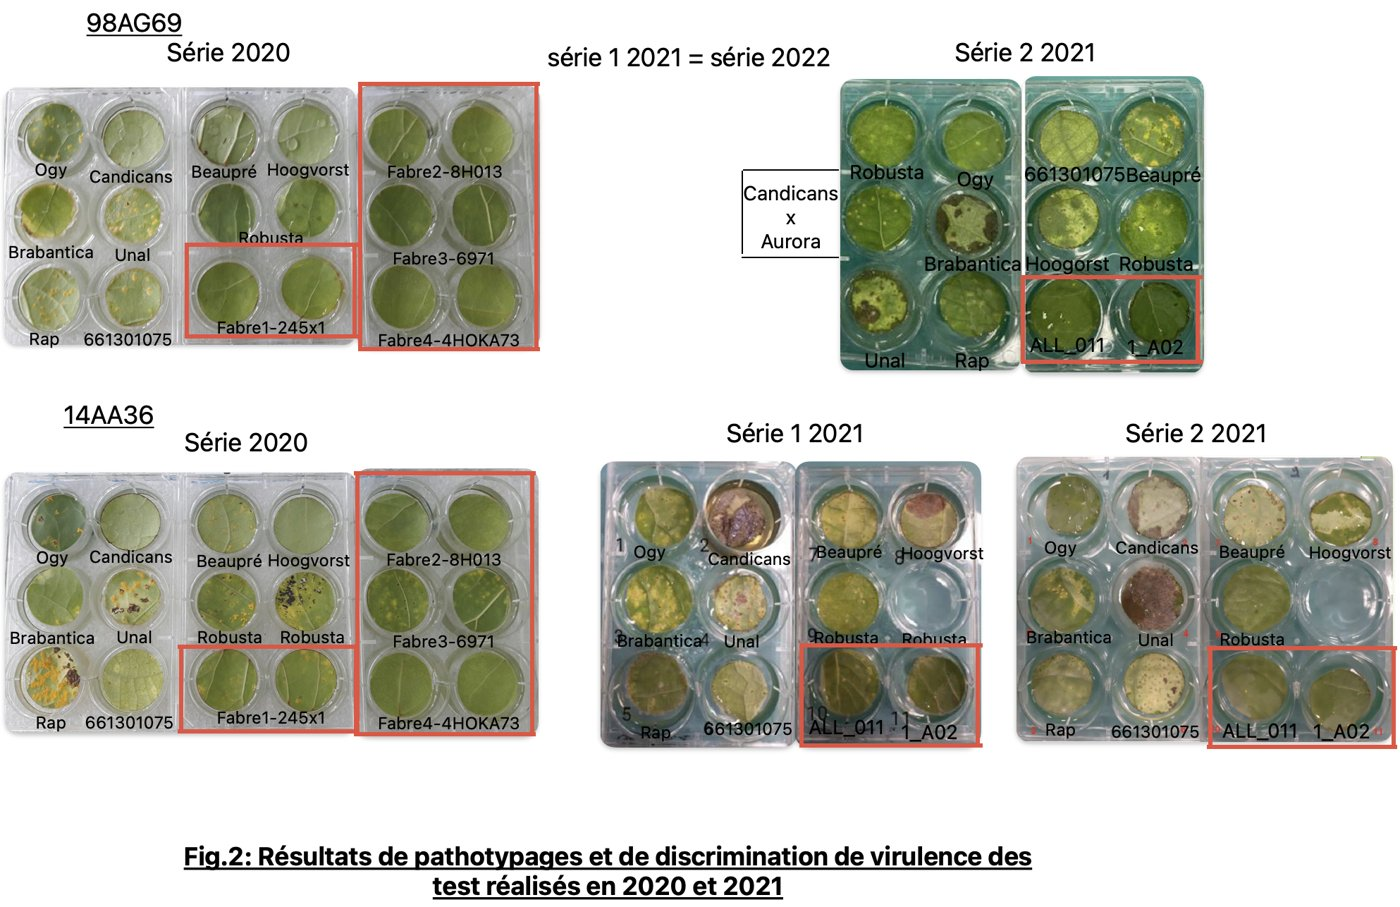
\includegraphics[width=0.85\linewidth]{figures/s04_1.jpg}
\caption{Disques foliaires après inoculation, séries 2020 et 2021 (en haut : 98AG69 ; en bas : 14AA36).}
\label{fig:plaques}
\end{figure}

\subsubsection{Interprétation}
Pour \textbf{14AA36}, le témoin Robusta n'est infecté qu'en 2020 : seule cette série est pleinement interprétable. Des sores apparaissent sur Ogy, Brabantica, Unal, Rap et Beaupré, mais pas sur Candicans × Aurora, 661301075-84B09 ni Hoogvorst. La souche porte donc les virulences 1, 3, 4, 5 et 7 : son pathotype est \textbf{1-3-4-5-7}. Les séries de 2021, sans infection du témoin, montrent tout de même des sores sur les clones 1, 3, 4 et 7, ce qui va dans le même sens.

Pour \textbf{98AG69}, Robusta n'est infecté dans aucune série. Des sores apparaissent pourtant sur plusieurs différentiels, mais pas les mêmes d'une année à l'autre (1, 4, 5 et 6 en 2020 ; 2 et 7 en 2021) : le pathotype ne peut pas être établi. L'absence d'infection du témoin peut venir de la viabilité des spores, des conditions d'incubation ou de la manipulation des disques.

Ces conclusions reposent sur une seule série valide par souche : seules des répétitions indépendantes, avec un témoin infecté à chaque fois, permettraient de confirmer les pathotypes.

\subsection{Sensibilité de nouveaux clones}
\subsubsection{Dispositif}
Le même protocole est appliqué à des clones de résistance inconnue, avec Robusta comme témoin (figure~\ref{fig:dispositif2}). En 2020, chaque clone est testé deux fois dans un même essai (répétitions) ; en 2021, l'essai entier est refait deux fois (séries).

\begin{figure}[ht]
\centering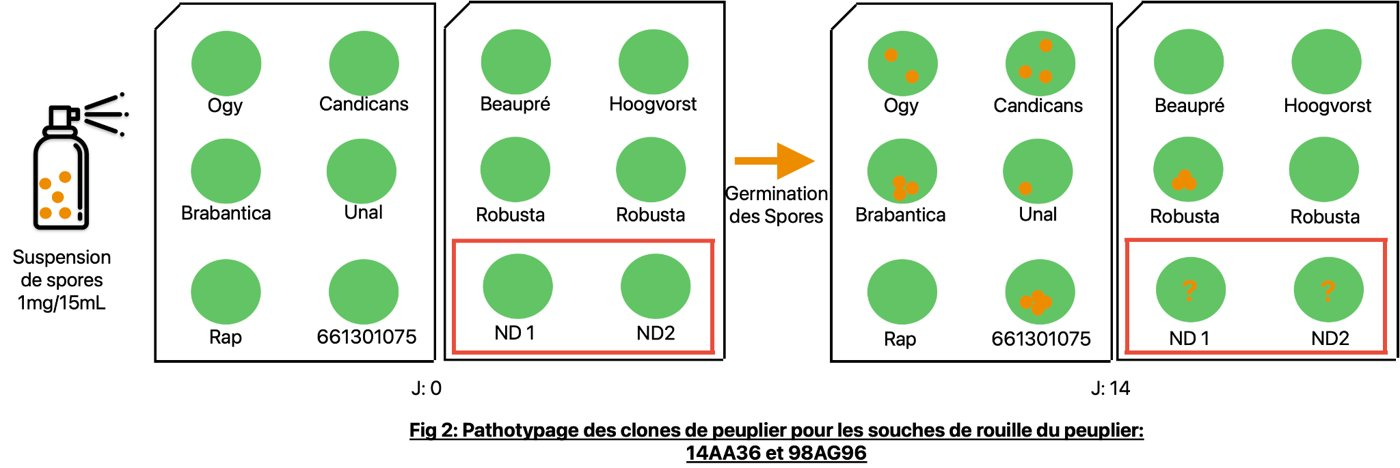
\includegraphics[width=0.85\linewidth]{figures/s08_1.jpg}
\caption{Dispositif de discrimination : les clones à caractériser remplacent les différentiels.}
\label{fig:dispositif2}
\end{figure}

\subsubsection{Résultats et interprétation}
Avec 98AG69, aucun clone n'est infecté, témoin compris : le test n'est pas interprétable. Avec 14AA36, seule la première répétition de 2020 infecte le témoin (tableau~\ref{tab:discri}). Fabre1-245x1 et Fabre3-6971 portent des sores dans les deux répétitions : ils sont \textbf{sensibles} à 14AA36. Fabre2-8H013 et Fabre4-4HOKA73 n'en portent aucun : ils sont \textbf{résistants}.

Un clone sensible ne porte aucun gène de résistance efficace contre 14AA36 : il peut posséder des gènes R1, R3, R4, R5 ou R7, que la souche contourne, ou aucun. Un clone résistant porte au moins un gène que 14AA36 ne contourne pas, R2, R6, R8 ou un gène encore inconnu. Les tests de 2021 (ALL\_011 et 1\_A02) ne sont pas interprétables, le témoin n'ayant pas été infecté.

\begin{table}[ht]
\centering\small
\caption{Discrimination de clones de résistance inconnue : classe de nombre de sores et taille (p : petits) par répétition (2020) ou série (2021) ; n.d. : non déterminé.}
\label{tab:discri}
\begin{tabular}{@{}lccl@{}}
\toprule\entete
Clone (année) & 14AA36 & 98AG69 & Conclusion pour 14AA36\\
\midrule
Robusta (2020), témoin & 4 p / 0 & 0 / 0 & témoin infecté une fois\\
Fabre1-245x1 (2020) & 3 p / 3 p & 0 / 0 & sensible\\
Fabre2-8H013 (2020) & 0 / 0 & 0 / 0 & résistant\\
Fabre3-6971 (2020) & 2 p / 2 p & 0 / 0 & sensible\\
Fabre4-4HOKA73 (2020) & 0 / 0 & 0 / 0 & résistant\\
\midrule
Robusta (2021), témoin & 0 / 0 & n.d. / 0 & témoin non infecté\\
ALL\_011 (2021) & 0 / 1 & n.d. / 0 & non interprétable\\
1\_A02 (2021) & 0 / 0 & n.d. / 0 & non interprétable\\
\bottomrule
\end{tabular}
\end{table}

\subsubsection{Perspectives}
La gravité des symptômes dépend à la fois de l'agressivité de la souche et du niveau de résistance du clone. Il faudrait répéter ces tests sur les clones sensibles, et sur des souches de pathotypes variés, pour vérifier la stabilité des réactions. L'enjeu de la sélection est de combiner des résistances que les souches présentes ne contournent pas, sans exercer une pression de sélection qui favoriserait l'émergence de nouvelles virulences, tout en conservant la productivité du peuplier \parencite{pinon2005}.

\section{Reconnaissance de maladies et de dégâts}
Ces fiches rassemblent les échantillons observés en TP, à l'œil nu, à la loupe binoculaire et au microscope. Pour chacun, on identifie l'agent, l'hôte et les symptômes diagnostiques \parencite{agrios2005,lepoivre2003}.

\noterevision{Note de révision (2026) : plusieurs fiches de 2023 ont été corrigées. Les taches noires du rosier et la nécrose foliaire sont dues à des champignons, pas à des virus. La galle du tilleul est causée par un acarien. Le feu bactérien est dû à \emph{Erwinia amylovora} : la fiche d'origine décrivait \emph{Fusarium circinatum}, champignon du pin. Enfin, la rouille hébergée par l'épine-vinette est la rouille noire (\emph{Puccinia graminis}), et non la rouille brune (\emph{P. triticina}).}

\needspace{18\baselineskip}\subsection*{Champignons}
\fiche{Oïdium du chêne}{\ph{s12_4.jpg}\ph{s12_1.jpg}\ph{s12_2.jpg}}
 {\emph{Erysiphe alphitoides}, plus rarement \emph{E. quercicola} \parencite{wikioidium}}
 {chênes à feuilles caduques, surtout pédonculé et sessile ; jeunes pousses et rejets}
 {feutrage blanc poudreux sur les feuilles, visible à l'œil nu ; déformation, jaunissement et chute précoce des feuilles}{}

\fiche{Oïdium des cucurbitacées}{\ph{s13_2.jpg}\ph{s13_1.jpg}}
 {\emph{Podosphaera xanthii} et \emph{Golovinomyces cichoracearum}}
 {courges et autres cucurbitacées}
 {feutrage blanc sur les deux faces des feuilles ; au microscope, conidies en chaînes ; jaunissement et sénescence précoce}{}

\fiche{Oïdium du noisetier}{\ph{s14_1.jpg}\ph{s14_2.jpg}}
 {\emph{Erysiphe corylacearum}}
 {noisetier (\emph{Corylus avellana})}
 {feutrage blanc sur les feuilles, jaunissement et sénescence précoce}{}

\fiche{Oïdium de la vigne}{\ph{s15_1.jpg}\ph{s15_2.jpg}}
 {\emph{Erysiphe necator}}
 {vigne (\emph{Vitis vinifera})}
 {feutrage blanc grisâtre sur les feuilles et les grappes, taches brunes, jaunissement des feuilles}{}

\fiche{Rouille grillagée du poirier}{\ph{s16_4.jpg}\ph{s16_2.jpg}\ph{s16_3.jpg}}
 {\emph{Gymnosporangium sabinae} (syn. \emph{G. fuscum}), rouille à deux hôtes}
 {poirier (\emph{Pyrus communis}) pour la phase à écidies ; genévriers pour la phase hivernale}
 {taches orange vif sur la face supérieure des feuilles ; à la face inférieure, excroissances portant des écidies en cornets ajourés (d'où le nom de rouille grillagée)}{}

\fiche{Cloque du pêcher}{\ph{s17_1.jpg}\ph{s17_2.jpg}}
 {\emph{Taphrina deformans}}
 {pêcher (\emph{Prunus persica})}
 {feuilles boursouflées, enroulées et rougies au printemps, puis desséchées ; au microscope, hyphes et asques à la surface des feuilles}{}

\fiche{Ergot du seigle}{\ph{s18_1.jpg}\ph{s18_2.jpg}\ph{s18_3.jpg}}
 {\emph{Claviceps purpurea}}
 {seigle (\emph{Secale cereale}) et nombreuses graminées}
 {sclérotes noirs et allongés à la place des grains de l'épi ; riches en alcaloïdes toxiques (ergotisme)}{}

\fiche{Rouille du peuplier}{\ph{s19_1.jpg}\ph{s19_2.jpg}}
 {\emph{Melampsora larici-populina} (hôte alternant : mélèze) et \emph{M. allii-populina} (hôte alternant : ail)}
 {peupliers (\emph{Populus})}
 {pustules orange (urédies) à la face inférieure, taches jaunes à la face supérieure ; défoliation précoce, mauvais aoûtement des rameaux, croissance réduite}{}

\fiche{Fusariose vasculaire de la tomate}{\ph{s20_1.jpg}\ph{s20_2.jpg}}
 {\emph{Fusarium oxysporum} f. sp. \emph{lycopersici}}
 {tomate (\emph{Solanum lycopersicum})}
 {jaunissement unilatéral puis nécrose des feuilles, flétrissement, brunissement des vaisseaux et dégâts racinaires}{}

\fiche{Rouille noire du blé}{\ph{s21_1.jpg}\ph{s21_2.jpg}\ph{s21_3.jpg}}
 {\emph{Puccinia graminis} f. sp. \emph{tritici}}
 {blé (\emph{Triticum}) et épine-vinette (\emph{Berberis vulgaris}), hôte alternant}
 {pustules couleur rouille puis noires sur tiges et feuilles du blé. Sur l'épine-vinette, écidies libérant des écidiospores dicaryotiques qui infectent le blé ; les urédospores (dicaryotiques) multiplient la maladie sur le blé ; les téleutospores (diploïdes) germent en basidiospores haploïdes qui infectent l'épine-vinette}{}

\fiche{Charbon du maïs}{\ph{s22_2.jpg}\ph{s22_1.jpg}\ph{s22_3.jpg}}
 {\emph{Ustilago maydis}}
 {maïs (\emph{Zea mays})}
 {galles blanchâtres sur épis, tiges et feuilles, qui éclatent en libérant une poudre noire de téliospores}{}

\fiche{Moniliose}{\ph{s23_1.jpg}\ph{s23_2.jpg}}
 {\emph{Monilinia fructigena} ou \emph{M. laxa}}
 {pommier (\emph{Malus domestica}) et autres arbres fruitiers}
 {pourriture brune des fruits avec coussinets de spores en cercles concentriques, momification des fruits ; dessèchement et chancres sur rameaux}{}

\fiche{Maladie des taches noires du rosier}{\ph{s34_1.jpg}\ph{s34_2.jpg}}
 {\emph{Diplocarpon rosae} (forme asexuée \emph{Marssonina rosae}), un champignon}
 {rosiers (\emph{Rosa})}
 {taches noires arrondies à bord frangé sur les feuilles, jaunissement puis chute des feuilles ; affaiblissement de la plante}{}

\fiche{Nécrose foliaire sur érable}{\ph{s32_1.jpg}\ph{s32_2.jpg}}
 {champignon probable, non identifié}
 {feuille identifiée en 2023 comme platane ; la forme des lobes évoque plutôt l'érable plane (\emph{Acer platanoides})}
 {tache nécrotique brune à halo jaune, près des nervures, portant de petites ponctuations noires (fructifications)}
 {Les ponctuations noires orientent vers un champignon ; une culture ou une observation microscopique des fructifications serait nécessaire pour conclure.}

\needspace{18\baselineskip}\subsection*{Insectes et acariens}
\fiche{Galle du chêne}{\ph{s24_1.jpg}\ph{s24_2.jpg}\ph{s24_3.jpg}}
 {cynipidé (hyménoptère), \emph{Neuroterus quercusbaccarum}}
 {chênes (\emph{Quercus})}
 {galles sur les feuilles : tissus de l'hôte hypertrophiés sous l'action de l'insecte, qui abritent et nourrissent la larve}{}

\fiche{Galle de la ronce}{\ph{s25_1.jpg}\ph{s25_2.jpg}\ph{s25_3.jpg}}
 {cécidomyie (diptère), \emph{Lasioptera rubi}}
 {ronces (\emph{Rubus})}
 {renflement de la tige ; en coupe, cavités occupées par les larves}{}

\fiche{Bédégar du rosier}{\ph{s26_1.jpg}\ph{s26_2.jpg}\ph{s26_3.jpg}}
 {cynipidé (hyménoptère), \emph{Diplolepis rosae}}
 {églantier et rosiers (\emph{Rosa})}
 {galle chevelue faite de filaments enchevêtrés, au centre dur abritant de nombreuses loges larvaires}{}

\fiche{Galle du tilleul}{\ph{s27_1.jpg}\ph{s27_4.jpg}\ph{s27_5.jpg}}
 {acarien ériophyide, \emph{Eriophyes tiliae}}
 {tilleuls (\emph{Tilia})}
 {petites galles rougeâtres sur la face supérieure des feuilles, ouvertes à la face inférieure}{}

\needspace{18\baselineskip}\subsection*{Plantes parasites}
\fiche{Gui}{\ph{s28_3.jpg}\ph{s28_1.jpg}\ph{s28_2.jpg}}
 {\emph{Viscum album}, plante hémiparasite}
 {nombreux feuillus et certains résineux, selon la sous-espèce}
 {touffes persistantes sur les branches ; le gui fait sa propre photosynthèse mais prélève l'eau et les sels minéraux de l'hôte par un suçoir (haustorium) ; dépérissement de l'hôte en cas de forte densité}{}

\fiche{Cuscute}{\ph{s29_2.jpg}\ph{s29_1.jpg}}
 {\emph{Cuscuta} sp., plante holoparasite sans chlorophylle}
 {nombreuses plantes, dont luzerne, lin et pomme de terre}
 {tiges filamenteuses jaunes à orangées enroulées autour de l'hôte, fixées par des haustoria ; baisse de rendement}{}

\needspace{18\baselineskip}\subsection*{Bactéries}
\fiche{Feu bactérien}{\ph{s30_1.jpg}\ph{s30_2.jpg}\ph{s30_3.jpg}}
 {\emph{Erwinia amylovora}, bactérie réglementée}
 {rosacées à pépins : poirier, pommier, aubépine, cotonéaster}
 {rameaux recourbés en crosse, feuilles et fleurs noircies qui restent attachées comme brûlées ; chancres et exsudats bactériens}{}

\fiche{Galle du collet}{\ph{s31_1.jpg}\ph{s31_2.jpg}}
 {\emph{Agrobacterium tumefaciens}, qui transfère à la plante un fragment d'ADN (ADN-T) déclenchant la prolifération des cellules}
 {très polyphage ; observé ici sur tabac (\emph{Nicotiana tabacum})}
 {tumeurs sur la tige et au collet}{}

\needspace{18\baselineskip}\subsection*{Virus}
\fiche{Mosaïque du châtaignier}{\ph{s33_2.jpg}\ph{s33_3.jpg}\ph{s33_1.jpg}}
 {virus non identifié en TP}
 {châtaignier (\emph{Castanea sativa})}
 {marbrures jaunes en mosaïque sur le limbe, plages nécrosées}
 {La version de 2023 attribuait la maladie au puceron \emph{Myzocallis castanicola} : ce puceron est un ravageur du châtaignier, pas l'agent d'une mosaïque ; son rôle de vecteur n'a pas été vérifié.}

\fiche{Nécrose virale du châtaignier}{\ph{s35_1.jpg}\ph{s35_3.jpg}\ph{s35_2.jpg}}
 {virus présumé, non identifié}
 {châtaignier (\emph{Castanea sativa})}
 {taches nécrotiques et jaunissement du limbe}
 {L'origine virale n'est qu'une hypothèse : elle demanderait un test sérologique ou moléculaire.}

\pagebiblio
\end{document}
